\documentclass[12pt,a4paper]{article}
\usepackage[utf8]{inputenc}
\usepackage[ngerman]{babel}
\usepackage{hyperref}
\usepackage[T1]{fontenc}
\usepackage{amsmath}
\usepackage{amsfonts}
\usepackage{amssymb}
\usepackage{graphicx}
\author{Jonathan Weißenberger}
\title{Projektbeschreibung/Aufgabenbeschreibung}
\begin{document}
\maketitle
\newpage
\tableofcontents
\newpage
\section{Allgemeine Beschreibung}
Das Team, bestehend aus Alexander Hebel, Dennis Seilnacht und Jonathan Weißenberger beschäftigen sich im vierten Semester mit der Portierung der Umgebung OpenPEARL für Microcontroller. Das Target in der Portierung ist das Entwicklungsboard STM32F746-DISCO. Zusätzlich zur Portierung erfolgt eine Demoapplikation. Hierbei ist die bereits existierende Kugelsortierungsanlage der Hochschule Furtwangen mit dem Microcontrollerboard zu steuern.
\begin{figure}[h]
\begin{center}
\caption{Kugelsortiermaschine}
\label{bild_kugelsortiermaschine}
\end{center}
\end{figure}

Das primäre Ziel der Arbeit ist die Lauffähigkeit von OpenPEARL auf der Zielplattform. Im Konkreten bedeutet das, dass Software in der Sprache OpenPEARL übersetzt werden kann und dann nach der Übertragung auf dem Zielsystem läuft. Das Kompilat soll nachvollziehbare Ergebnisse liefern, die wir zuvor definieren. Im Fall der Sortierungsanlage sollen die Kugeln ihrer jeweiligen Dichte entsprechend in die einzelnen Fächer eingeordnet werden. Die Dichte errechnet sich dann aus dem Durchmesser der Kugel und dem Gewicht ($Dichte=Masse/Volumen$). Zu den Funktionalitäten, die mit OpenPEARL genutzt werden sollen gehört das $I^2C$-Bussystem. Durch das Bussystem wird die Kugelsortierungsmaschine angesteuert und Informationen abgerufen. Außerdem soll eine Kommunikationsverbindung mit dem Target mittels UART-Schnittstelle von einem Host-Computer aus möglich sein. Durch die Schnittstelle soll es möglich sein, Befehle an den Microcontroller zu senden und Informationen abzurufen. 
\begin{figure}[h]
\begin{center}
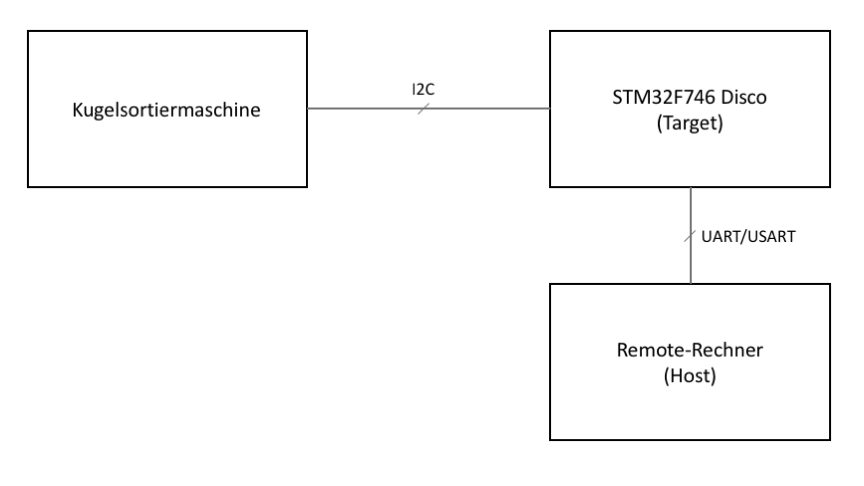
\includegraphics[width=10cm]{grafiken/Schematik.png}
\caption{Schematik des Projektaufbaus}
\label{schematik_projektaufbau}
\end{center}
\end{figure}
Sofern die Grundfunktionalitäten in angemessener Zeit umgesetzt werden können, wird zusätzlich die Verwendbarkeit des Displays angestrebt. Das Display soll zusätzlich Statusberichte liefern über den Zustand der Sortierungsanlage. 
\end{document}